\section{Memory Optimizations}

\section{Vector Instructions}
\cuda support vector accelerated memory operations of size 2, 3 and 4.
This means that we can load multiple values from memory in a single instruction.
This requires the data to be alagned to the size of the vector instruction.
For float instructions this is 8 bytes for float2 and 16 bytes for both float3 and float4.
As we also want acces patterns to be coalesced, we use the following memory layouts.

Caspar autogenerates all the code needed to map between the different memory layouts.

\begin{figure}[H]
    \centering
    \begin{tabular}[b]{ccc}
        \subcaptionbox{Array of scalars}{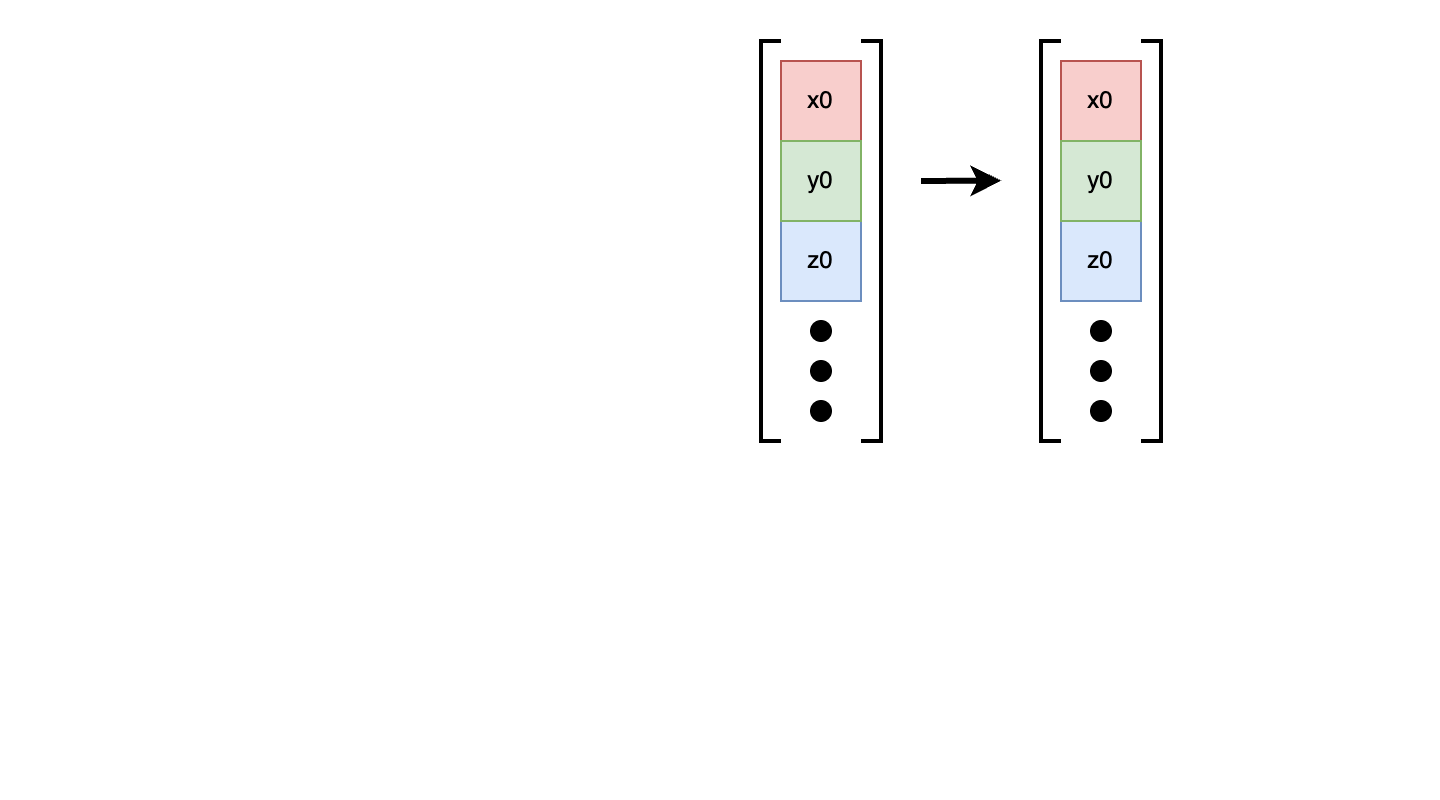
\includegraphics[trim={14cm 12cm -4cm 1cm},clip,width=0.5\textwidth]{figures/memlayouts/memlayout-1.png}
        } &
        \subcaptionbox{Array of structs with 3 fields.}{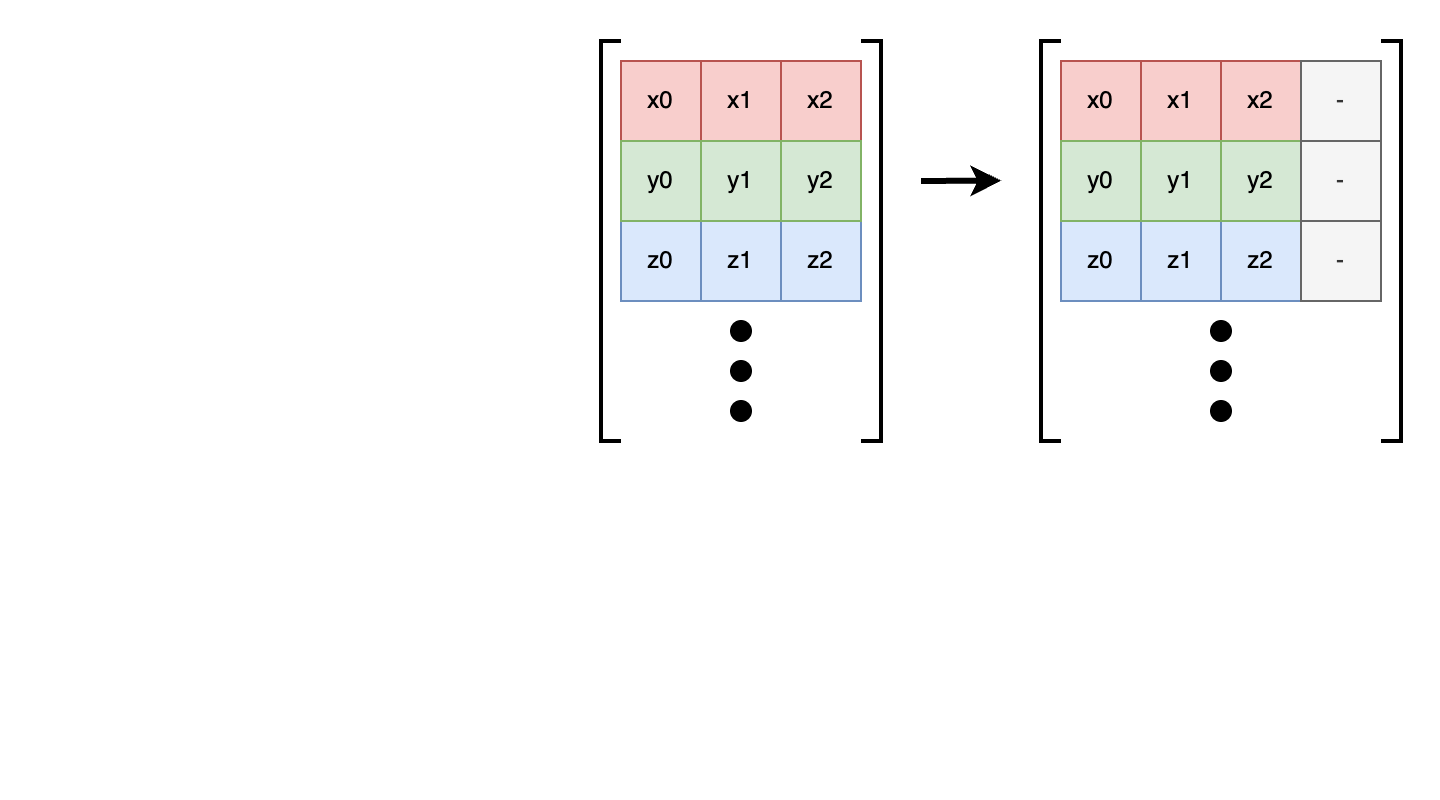
\includegraphics[trim={13cm 12cm -3cm 1cm},clip,width=0.5\textwidth]{figures/memlayouts/memlayout-3.png}
        }              \\
        \vspace{0.5cm} \\
        \subcaptionbox{Allay of structs with 6 fields.}{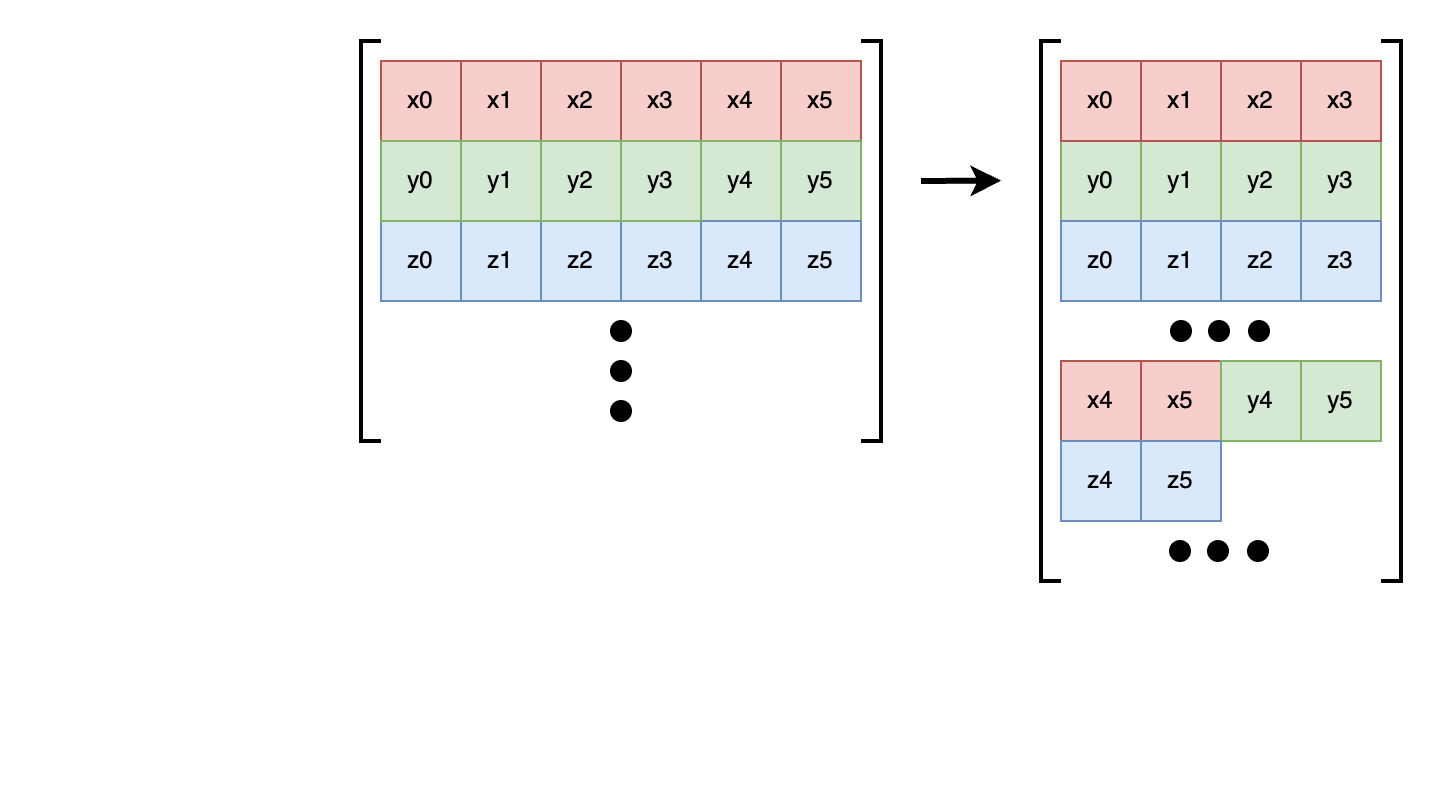
\includegraphics[trim={10cm 4cm 0cm 1cm},clip,width=0.5\textwidth]{figures/memlayouts/memlayout-6.png}
        } &
        \subcaptionbox{Array of structs with 7 fields.}{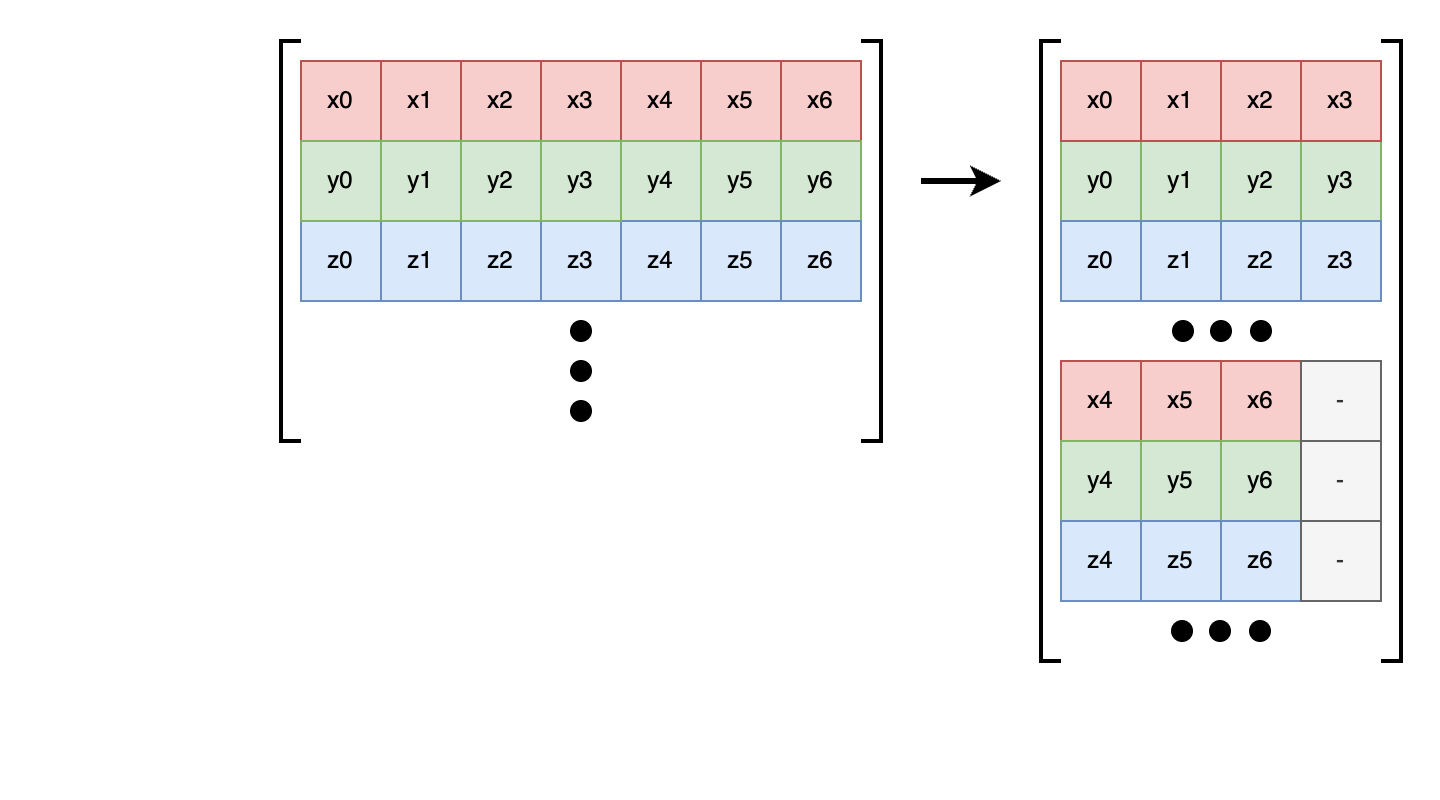
\includegraphics[trim={9cm 4cm 1cm 1cm},clip,width=0.5\textwidth]{figures/memlayouts/memlayout-7.png}
        }              \\
    \end{tabular}
    \caption{Mapping of arrays of structs with different number of fields. Fields are grouped into chunks of four as far as possibe, the remaning fields are appended at the end as chunks of the remaning size. All chunks are aligned to the number of bytes needed for the corresponding vector instruction.}
\end{figure}


\section{Access Patterns}
\subsection{Secuentual Acces}
\subsection{Indexed Acces}
\subsection{Shared Indexed Acces}

\subsection{Secuentual Add}
\subsection{Indexed Add}
\subsection{Shared Indexed Add}

\subsection{Unique Access}
